\subsection{Learning Performance}
In addition to reporting the performance of our complete method on various tasks, here we also report the training and validation accuracies of our learned models. Further details on the training of these models can be found in Sections ``\nameref{Scirob:sec:learning_dynamics}'', ``\nameref{Scirob:sec:learning_classifier}'', and ``\nameref{Scirob:sec:learning_recovery}''.

For dynamics learning, we report learning error as the Euclidean distance between every predicted and true point on the rope, and average over all the points, time steps, and examples in the dataset. For rope dragging, our unconstrained dynamics model has an error of \SI{0.0081}{\meter} in training and \SI{0.0097}{\meter} in testing. These numbers are small in comparison to the length of the rope (\SI{0.5}{\meter}) and the size of the environment (2x2m). For a visual demonstration of this level of error,r please see our video. FD achieves an error of \SI{0.0090}{\meter} in training and \SI{0.0117}{\meter} in testing. For dual arm rope manipulation, our unconstrained dynamics model has an error of \SI{0.0025}{\meter} in training in \SI{0.0030}{\meter} in testing. Here the rope has a length of \SI{0.8}{\meter}, indicating that we are able to learn the unconstrained dynamics very accurately. The full dynamics baseline achieves an error of \SI{0.0194}{\meter} in training and \SI{0.0218}{\meter} in testing. Learning accurate dynamics over long horizons is critical for planning, and by learning only the unconstrained dynamics, our method is able to do so with higher accuracy than the full dynamics baseline.

We report learning metrics on the phase two dataset (see Section ``\nameref{Scirob:sec:learning_classifier}'' for details). For rope dragging, the classifier achieved an accuracy of $0.890$, precision of $0.959$ and recall of $0.822$ on the training set. On the testing set, it has an accuracy of $0.835$, precision of $0.888$, and recall of $0.789$. For dual arm rope manipulation, the classifier achieved an accuracy of $0.904$, precision of $0.914$ and recall of $0.927$ on the training set. On the testing set, it has an accuracy of $0.890$, precision of $0.895$, and recall of $0.927$. Throughout our experimentation we observed that, as prior work has noted \cite{McConachie2020}, the accuracy of this classifier is a poor indicator of its usefulness in planning.

For recovery, we use the binary cross entropy loss to measure learning performance. For rope dragging, the training loss (unitless) is $0.021$ and the testing loss is $0.023$. For rope dragging, the training loss is $0.139$ and the testing loss is $0.146$. 

\subsection{Physical Robot Demonstrations}
\label{Scirob:sec:physical_robot_details}
To demonstrate the practicality of our method, we designed real-world mockups of domestic and automotive tasks. For dual arm manipulation, we demonstrate three tasks done under the hood of a car, where the robot manipulates hoses and straps. For rope dragging we show an example where the robot retrieves a phone charging cable by sliding it. For clarity and simplicity, we demonstrate only the parts of these tasks where our method applies and forgo the use of sophisticated local controllers to, for example, plug the charging cable into the phone.

Perception of deformable objects remains a difficult open problem \cite{Yan2020}, much less in cluttered environments where the object is partially-occluded. Online perception of the object is not within the scope of this paper. To demonstrate our methods despite not having such perception algorithms, we manually constructed the scenes in a simulator and planned our actions there before executing them on the real robot. In future work we will incorporate online perception into our execution pipeline when the appropriate perception algorithms are available.

In both scenes, we re-use the unconstrained dynamics models learned in simulation directly. For rope dragging, we also re-use the classifier and recovery models as-is. For dual arm manipulation however, because a different robot is used, and the scene geometry differs significantly from our simulation, we use classifier and recovery models trained on scenes similar to the one we test on in the real world.  For more information, see the video in our supplemental materials. 

\subsection{Experiment Design}
To compare these methods quantitatively, we consider the task error over 150 trials per method in two types of rope manipulation tasks. The obstacle configurations are randomized before every trial, and each trial is allowed 180 seconds. During these 180 seconds, the method alternates between action selection and execution, where action selection is either planning or recovery. The trial is terminated if the goal is reached or the time limit is reached (see Figure \ref{Scirob:fig:figure1}, and Supplementary Materials for more details).

At the end of the trial, the final state is used to determine task error, and we report statistics of this error across the trials. A trial is a success if the final state error is below the goal threshold. Because tasks are generated randomly, some tasks will be impossible to achieve (e.g. the object cannot reach the goal because of a barrier), thus the absolute success rate is less informative than the difference in success rates between methods. When claims of statistical significance are made, a one-sided T-test is used and p-values are reported.

\section{Results}

To rigorously evaluate our approach, we perform statistical comparisons of our method vs. ablations and baselines in simulation over two types of rope manipulation tasks in 150 randomly-generated environments. We show that our approach greatly improves performance over learning the full dynamics as well as simply trusting the model learned in a simplified setting. We then demonstrate the practicality of our method for performing tasks on a real robot in domestic and automotive scenarios.

\subsection{Baselines}

In this work we argue that learning the dynamics for deformable objects in environments with constraints such as obstacles is difficult, and that we should instead learn only the unconstrained dynamics and a classifier to predict when those dynamics are valid. To support this claim we compare to a method which plans with a model of the full dynamics. We term this baseline Full Dynamics (FD), and we learn the dynamics using an approach similar to \cite{Nagabandi2018} (see Section ``\nameref{Scirob:sec:learning_dynamics}''). In FD, we learn the dynamics from a dataset collected in the same way as we collect data for our classifier (Section ``\nameref{Scirob:sec:phase_two_collection}''). Our method uses two phases of data collection, the data in each phase is used differently. Therefore, to make a fair comparison, the full dynamics baseline is trained on a dataset whose size is equal to our method's two datasets combined. Once trained, we plan with FD using the same Rapidly-exploring Random Tree (RRT) planner as in our method. However, unlike our method, FD requires no constraint checker (learned or otherwise), as anything we might consider a constraint is subsumed by the dynamics.

Additionally, we remove various components of our method to demonstrate the benefits they provide. We compare to a version called \textit{No Classifier}, which plans using our unconstrained dynamics but no constraint checker. Comparisons to this baseline show the benefit of using the classifier over simply trusting the unconstrained dynamics everywhere. We also compare to a version without recovery (\textit{Classifier}), and a method which takes random actions as its recovery policy (\textit{Classifier + Random Recovery}).

\subsection{Scenario 1: Rope Dragging}
 
Here we describe our results for the task of dragging a rope-like object along a surface among obstacles, as is shown in Figure \ref{Scirob:fig:figure1}a. Rope manipulation has numerous important applications including suturing and managing wires or hoses, and the rope dragging task requires long horizon planning for which our method is well-suited. The task is to place one end of a rope at a point while dragging the rope by the other end. This task is difficult because the system is highly under-actuated and the environment is cluttered. Task error is the Euclidean distance between the end of the rope and the goal point. The goal region is a sphere about the goal point with radius \SI{5}{\centi\meter}. This task illustrates the challenges of long horizon planning for deformable objects in cluttered scenes, and is challenging for existing methods. The practicality of our method is illustrated in our physical robot demonstrations.

The task error across 50 trials is shown in Figure \ref{Scirob:fig:figure6}a. Our complete method reached the goal 76\% of the time with a mean task error of \SI{4.48}{\centi\meter}. This is better than FD (32\% success, \SI{20.32}{\centi\meter} error) and No Classifier (60\% success, \SI{8.20}{\centi\meter} error) and is significant at p $< 0.001$. Additional numerical results are shown in Table \ref{Scirob:tab:dragging_results}. For this task, recovery was never needed, meaning that for all states from which the planner was run there was at least one action from that state which our classifier accepted as yielding an accurate prediction. The benefit of recovery actions is shown in the dual arm manipulation task below.

To show the ability of our classifier to learn difficult prediction functions, we also compare our results to a manually-engineered solution for this scenario. By inspecting the data of where the model tended to make errors, we found that, unsurprisingly, the model could not predict the effect of pushing/pulling the rope into obstacles but was fairly accurate when not in contact with obstacles or sliding along them (See Supplementary Materials for examples of sliding motion accepted by our classifier). To capture this predictive behavior with a rough approximation we used a collision checker to measure if the predicted state was penetrating into the obstacle in place of our learned classifier (as is done in \cite{Lamiraux2001}). Note that this is a scenario-specific method derived by using human intuition and an engineered collision-checker. While this intuition and hand engineered solution can be an effective solution for some tasks, changes in the task or object being manipulated often lead to additional tuning and engineering. For example, if the rope was very thick and the points defining the rope state (which are along the central axis of the rope) did not enter obstacles even when the rope was pressing into an obstacle, collision boundaries would need to be tuned. Likewise, if the rope is very thin, numerical error in predictions could lead to erroneous collision-checking results when sliding along the surface of an obstacle. To the credit of our method, we found that using the collision checker gave a 78\% success rate and a mean task error of \SI{12.74}{\centi\meter}, with p $= 0.498$ for the hypothesis that our method outperforms the collision checking method. This is an encouraging result, as it demonstrates that our method can perform on-par with a scenario-specific human-engineered solution, at least in this scenario.

\subsection{Scenario 2: Dual Arm Rope Manipulation}

\begin{figure}
    \centering
    \begin{subfigure}[b]{0.49\textwidth}
        \centering
        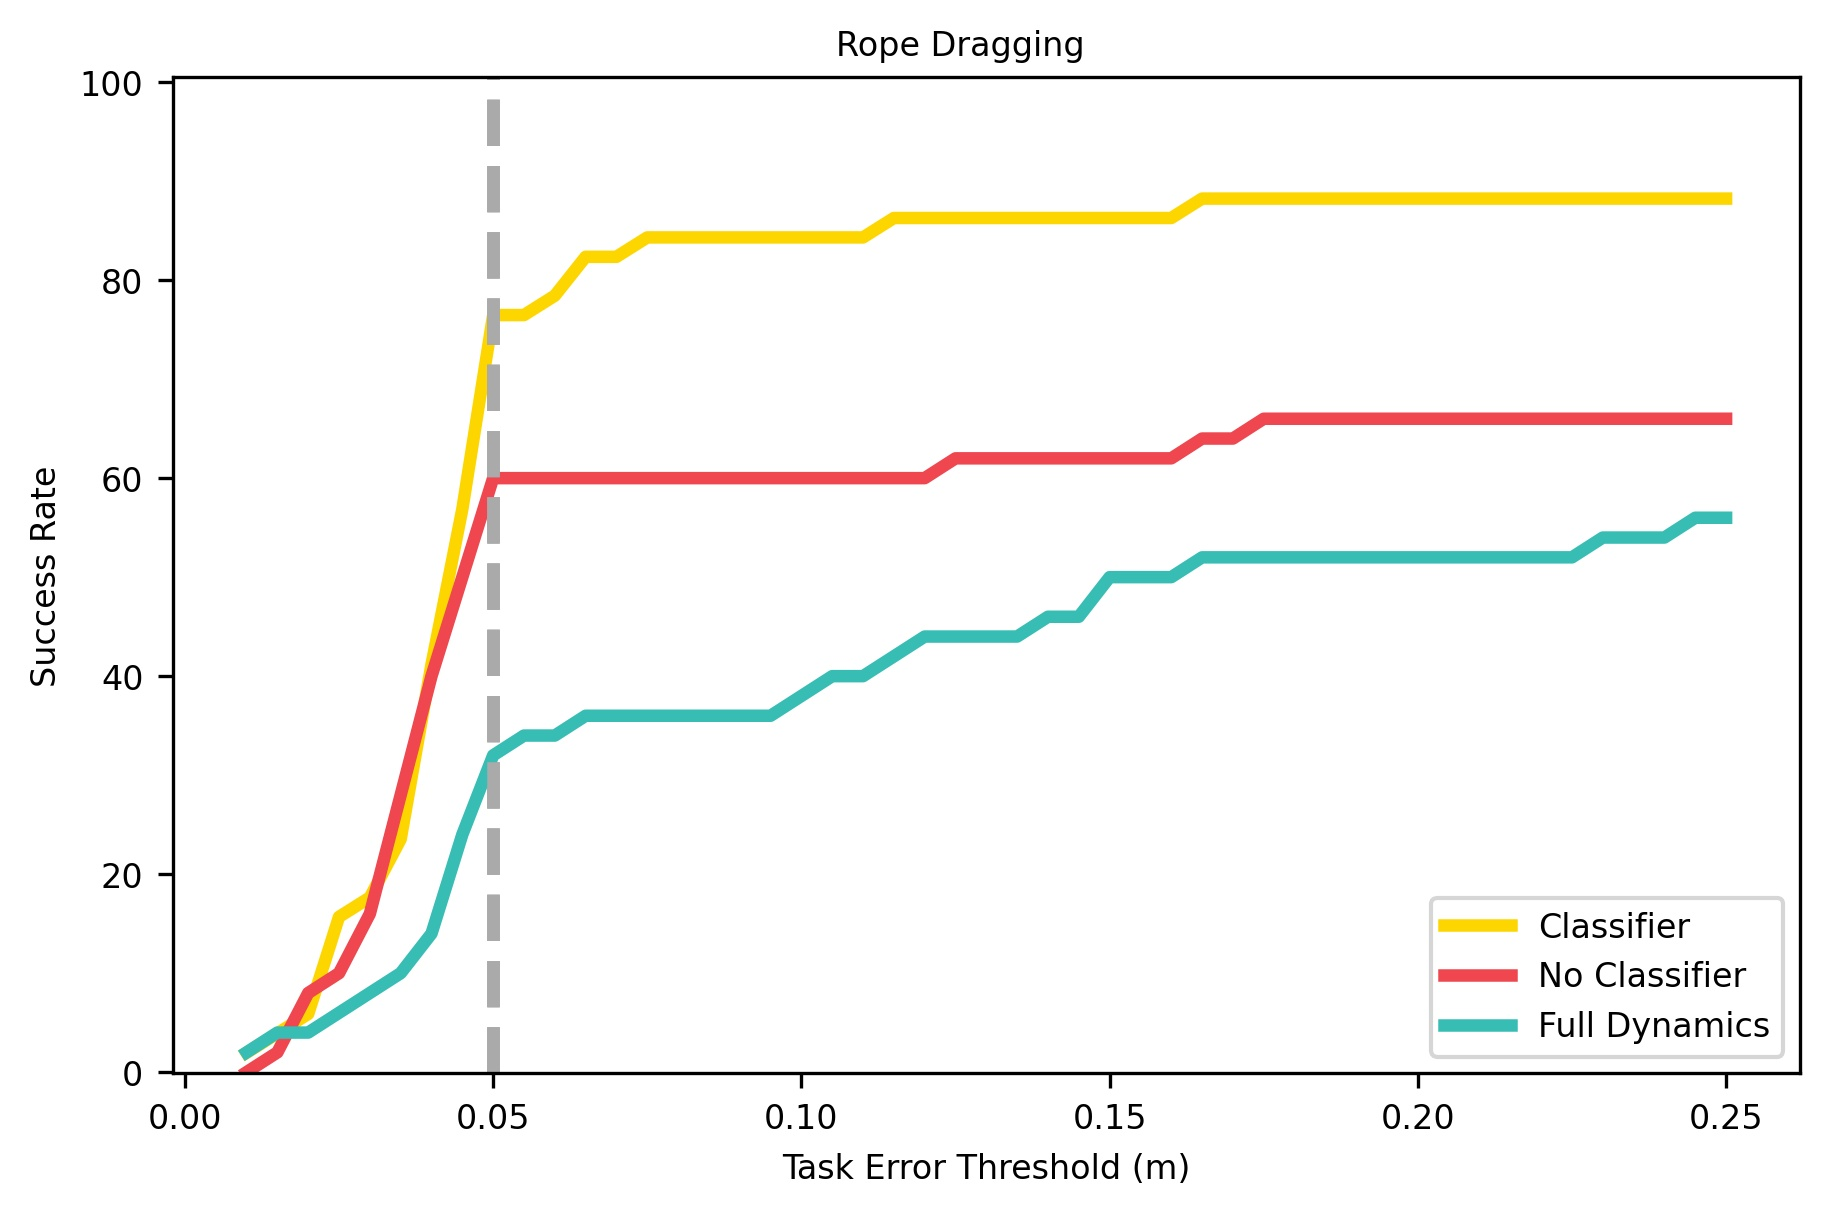
\includegraphics[width=\textwidth]{Chap2/images/dragging_success.jpeg}
        \label{Scirob:fig:dragging_success}
    \end{subfigure}
    \hfill
    \begin{subfigure}[b]{0.49\textwidth}
        \centering
        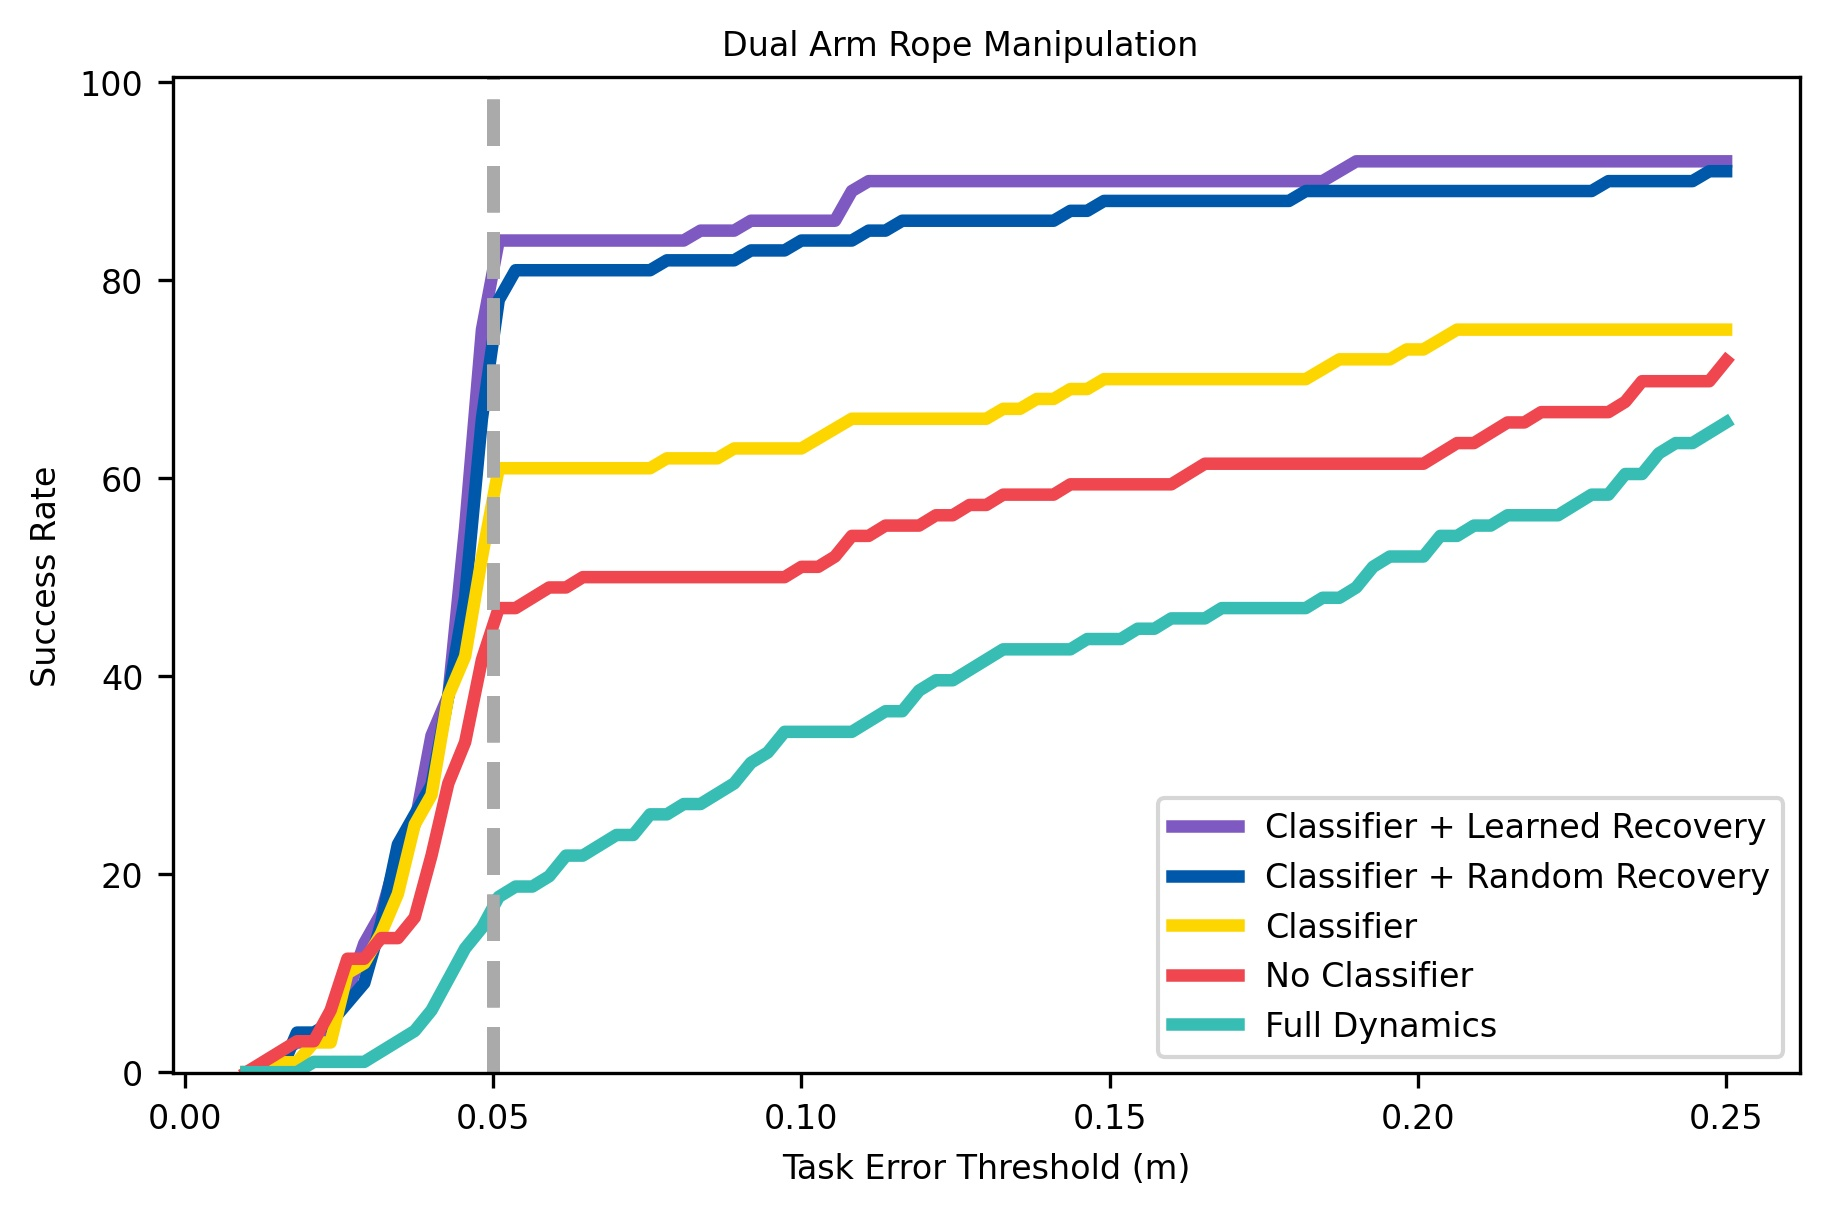
\includegraphics[width=\textwidth]{Chap2/images/dual_success.jpeg}
        \label{Scirob:fig:dual_success}
    \end{subfigure}
    \caption{Comparing success across methods. (left) The success rate as a function of the success threshold on task error for our simulated rope dragging experiments. The dashed line indicates the size of the goal region used. For example, this tells us that if our goal region was \SI{0.1}{\meter}, the "Classifier" method would achieve about 84\% success. (right) The success rate as a function of the success threshold on task error for our simulated dual arm rope manipulation experiments.}
    \label{Scirob:fig:figure6}
\end{figure}

Here we describe our results for using a robot for dual arm manipulation of rope among obstacles, as is shown in Figure \ref{Scirob:fig:figure2}b. Using two arms to manipulate deformable objects allows more control of the object than one arm and introduces additional interesting challenges in coordinating the two arms. The task we use for evaluation is to place the midpoint of the rope at a point in 3D while only holding the ends. In addition to obstacles, this scenario imposes the constraints of not overstretching the rope, not colliding the arms, and staying within the reachability limits of the robot. Task error is the Euclidean distance between the midpoint of the rope and the goal point. The goal region is defined as a sphere about the goal point with radius \SI{5}{\centi\meter}. This type of manipulation, while difficult for existing methods, is a prerequisite for many practical tasks such as cable harnessing.

The task error across 100 trials is shown in Figure \ref{Scirob:fig:figure6}b. Our complete method (\textit{Classifier + Learned Recovery}) reached the goal 84\% of the time with a mean task error of \SI{7.29}{\centi\meter}. This is statistically significantly (p $<0.001$) better than FD, which reached the goal 17.7\% of the time with a mean task error of \SI{20.32}{\centi\meter}, and No Classifier, which reached the goal 47\% of the time with a mean task error of \SI{16.97}{\centi\meter}. We also compare to our method without recovery actions, and to our method with random recovery actions. In this task, recovery actions are critical, and without them our method performs statistically significantly (p $<0.001$) worse with a success rate of 61\% and a mean task error of \SI{14.69}{\centi\meter}. When compared to random recovery actions, which reaches the goal 78\% of the time, our method has similar task error (p $= 0.281$ for the hypothesis that our method outperforms random recovery), however our method needs only a third as many recovery actions to achieve this task error. Over all 100 trials, random recovery used 613 recovery actions whereas our method used only 177. Additional numerical results are shown in Table \ref{Scirob:tab:dual_results}.

\subsection{Physical Robot Demonstrations}
We demonstrate potential applications of our method on real-world mock-ups of several domestic and automotive tasks. The first set of tasks are performed under the hood of a car, and require the robot to manipulate straps or hoses. These tasks include moving the midpoint of a hose to a specific location (Figure \ref{Scirob:fig:figure2}e), positioning the ends of a wiper fluid hose for installation (Figure \ref{Scirob:fig:figure2}f), and removing lifting straps from an engine (Figure \ref{Scirob:fig:figure2}d).

We also perform the task of fetching a charging cable (Figure \ref{Scirob:fig:figure2}c). In this example, the robot cannot reach the end of the cable directly because it is blocked by an obstacle. Instead, the robot grasps the cable elsewhere, and must drag the end of the cable towards the phone.

Notably, these tasks use several different types of goals described in the state space of the rope and grippers, all of which can be handled by our planner. This is in contrast to policy learning methods \cite{matas2018sim2real,Sundaresan2020,Wu2020} and methods which use goal images \cite{Nair2017,Finn2017,Zhang2019}. More details on how we perform these tasks can be found in Section ``\nameref{Scirob:sec:physical_robot_details}''.

\FloatBarrier

\begin{table}
    \centering
    \begin{tabular}{lllccccc}
    \hline\noalign{\smallskip}
     Name                        & Dynamics      & Classifier  & \makecell{max\\(m)} & \makecell{mean\\(m)} & \makecell{median\\(m)} & \makecell{std. dev.\\(m)} \\
    \noalign{\smallskip}\hline\hline\noalign{\smallskip}
     \makecell[l]{Classifier}    & Unconstrained & Learned     & 1.133   & 0.128    &  0.044     & 0.247 \\
     \noalign{\smallskip}\hline\noalign{\smallskip}
     \makecell[l]{No Classifier} & Unconstrained & None        & 1.408   & 0.325    &  0.045     & 0.425 \\
     \noalign{\smallskip}\hline\noalign{\smallskip}
     \makecell[l]{Full Dynamics} & Full          & None        & 1.519   & 0.438    &  0.156     & 0.450 \\
    \noalign{\smallskip}\hline
    \end{tabular}
    \caption{\label{Scirob:tab:dragging_results} Task error statistics for simulated rope dragging.}
\end{table}

\begin{table}
    \centering
    \begin{tabular}{lllccccc}
    \hline\noalign{\smallskip}
     Name                                        & Dynamics      & Classifier  & \makecell{max\\(m)} & \makecell{mean\\(m)} & \makecell{median\\(m)} & \makecell{std. dev.\\(m)} \\
    \noalign{\smallskip}\hline\hline\noalign{\smallskip}
     \makecell[l]{Classifier\\Learned\\Recovery} & Unconstrained & Learned    & 0.450   & 0.073    &  0.045     & 0.094 \\
     \noalign{\smallskip}\hline\noalign{\smallskip}
     \makecell[l]{Classifier\\Random\\Recovery}  & Unconstrained & Learned    & 0.629   & 0.081    &  0.046     & 0.106 \\
     \noalign{\smallskip}\hline\noalign{\smallskip}
     \makecell[l]{Classifier}                    & Unconstrained & Learned    & 0.630   & 0.147    &  0.047     & 0.167 \\
     \noalign{\smallskip}\hline\noalign{\smallskip}
     \makecell[l]{No Classifier}                 & Unconstrained & None       & 0.741   & 0.170    &  0.082     & 0.165 \\
     \noalign{\smallskip}\hline\noalign{\smallskip}
     \makecell[l]{Full Dynamics}                 & Full          & None       & 0.621   & 0.203    &  0.191     & 0.142 \\
    \noalign{\smallskip}\hline\noalign{\smallskip}
    \end{tabular}
    \caption{\label{Scirob:tab:dual_results}Task error statistics for simulated dual arm rope manipulation.}
\end{table}